\section{Results}

This section starts with the results of exploratory analysis of the data and subsequently details the results of the two aims of this project: understanding the behaviour of communities and users of speedrun.com, and creating a game recommendation system for speedrunners.

\subsection{Exploratory Analysis}

The cleansed data from speedrun.com was analysed to describe the characteristics and behaviour of the users on the platform. The data describes 332,746 users who had submitted 3,086,954 runs for 31,416 games. On average, a user on speedrun.com has 2.74 verified runs on only one game. 246,995 of these users (or 73.66\%) have only played one game, and similarly 138,300 users (41.54\%) have only achieved a single verified run. 


Metadata was collected for a total of 32,994 games from speedrun.com. The cleansed data set contained 31,405 games — all released before 2023 and contained no null values. The average game within this clean data has 4 categories, 7 levels, 88 runs, 19 users, and 2 guests. Ranking all games by the number of runs and number of users, the top game in both metrics is Seterra with 61,962 runs by 7,168 users. The data is very imbalanced, with 50\% of all games on speedrun.com having less than 10 runs, and the top 519 (or 1.65\% of) games have an equal number of runs to the bottom 30,886 (98.35\%) games. The game with the largest number of guests is Minecraft: Legacy Console Edition with 15,646 guests and 155 users; a highly unusual number of guests considering most games have higher numbers of users compared to guests.


The top three users have played 2059, 1884, and 916 different games respectively. This an unusually high number of unique games played with z-scores of 277.6, 254, and 123.3 respectively. Furthermore, ranking all users by the number of verified runs shows that the new top three users have 9800, 8822, and 7598 runs. These new top users do not necessarily have an abnormally high number of games played, as a few of these top users have a z-score of the number of games played $<1$.

\begin{figure}[h]
    \centering
    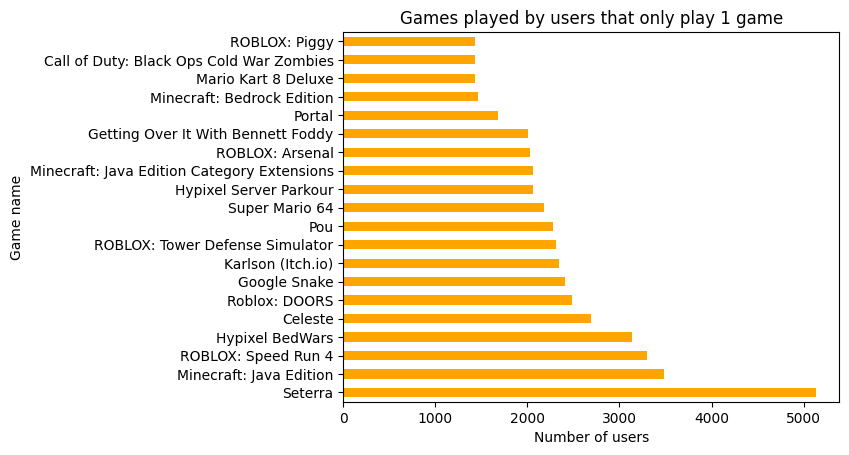
\includegraphics[width=0.7\linewidth]{images/user_onegame_preference.png}
    \label{fig:figure1}
    \caption{Games played by users on speedrun.com.}
\end{figure}

The most popular game for users that have played a single game is Seterra, an online map quiz game. The next largest games are Minecraft: Java Edition, ROBLOX: Speed Run 4, Hypixel BedWars, Celeste, ROBLOX: Doors, and Google Snake. Analysing the users that have only played two games, the pair of games that a user chooses to play seem to be related. Users play a combination of: a game and it's category extensions, a prequel/sequel to the first game, or a mini-game within the first game. For example, users that play Minecraft: Java Edition are likely to play games such as Minecraft: Java Edition Category Extensions (category extensions), Minecraft: Bedrock Edition (sequel), or any Hypixel game (mini-games). 

\begin{figure}[h]
    \centering
    \begin{subfigure}{0.45\linewidth}
        \centering
        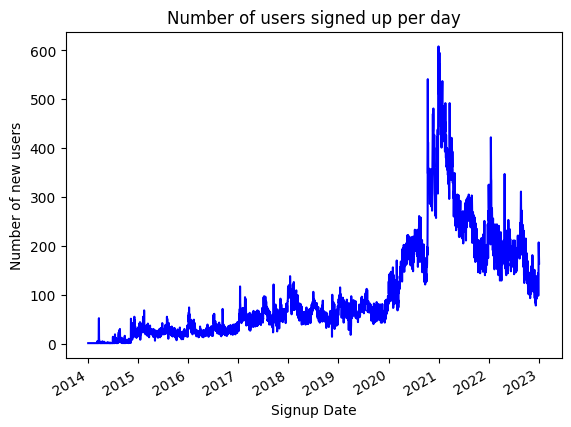
\includegraphics[width=\linewidth]{images/users_per_day.png}
        \caption{The number of new active users per day between 2014 and 2023.}
        \label{fig:figure1}
    \end{subfigure}
    \label{fig:figures}
    \hspace{0.05\linewidth}
    \begin{subfigure}{0.45\linewidth}
        \centering
        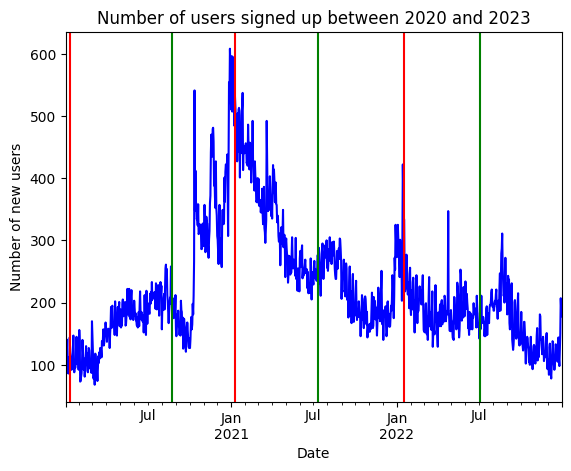
\includegraphics[width=\linewidth]{images/user_per_day_2020_2023.png}
        \caption{The number of new active users per day between 2020 and 2023. Dates of GDQ events highlighted in red and green.}
        \label{fig:figure2}
    \end{subfigure}
    \caption{Rate of new users joining speedrun.com and demographics of all users.}
    \label{fig:figures}
\end{figure}

The first user created their account on January 6th, 2014, and half of all users had created their accounts before January 4th, 2021. It took only two years to double the number of active users on speedrun.com. There is a massive increase in sign-ups starting around January 2020 and ending around January 2021. The average number of sign-ups per day is higher after the peak (232.2) than before (43.8). There are also short-term rises and falls in the number of sign-ups per year, with at least two specific increases in sign-ups.

\begin{figure}
    \centering
    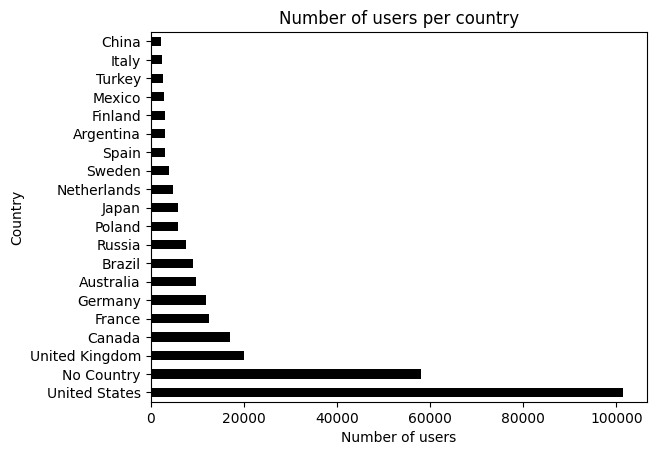
\includegraphics[width=0.5\linewidth]{images/user_demographics.png}
    \caption{The demographics of all active users of speedrun.com.}
    \label{fig:my_label}
\end{figure}

Focusing on the demographic metadata of the users, 101,439 users or (29.96\%) have submitted their location as the United States, making it the largest non-null demographic. The next largest demographic is `No Country Specified' with 58,107 (17.16\%) users, followed by the United Kingdom with 20,030 users (5.92\%). The subsequent demographics such as Canada, France, Germany, and Australia slowly decrease in the number of users.

\subsection{Network Analysis}

\renewcommand{\arraystretch}{1.2}
\begin{table}[h]
    \centering
    \begin{tabular}{|*{5}{C|}}
        \hline
        \textbf{Network Name} & \textbf{Number of Nodes} & \textbf{Number of Edges} & \textbf{Density} & \textbf{Clustering Coefficient} \\ \hline
        Game-Game & 30,433 & 14,739,311 & $1.59 \times 10^{-2}$ & 0.656 \\ \hline
        User-Game & 366,747 & 668,788 & $9.94 \times 10^{-6}$ & 0.496 \\ \hline
    \end{tabular}
    \caption{Comparison of the Game-Game and User-Game networks.}
    \label{tab:networks}
\end{table}

From the data collected two networks were created: a weighted and directed game-to-game network, and a directed bipartite user-to-game network. The game-game network has games as nodes, and weighted edges that are determined by the number of users that appear in a pair of games' leaderboards. This creates a network with 30,433 nodes and 14,739,311 edges. This network has a density of 0.0159, and a clustering coefficient of 0.657. There is a high degree distribution in the game-game network with a few very dominant nodes.

\begin{figure}[h]
  \centering
  \begin{subfigure}{0.45\linewidth}
    \centering
    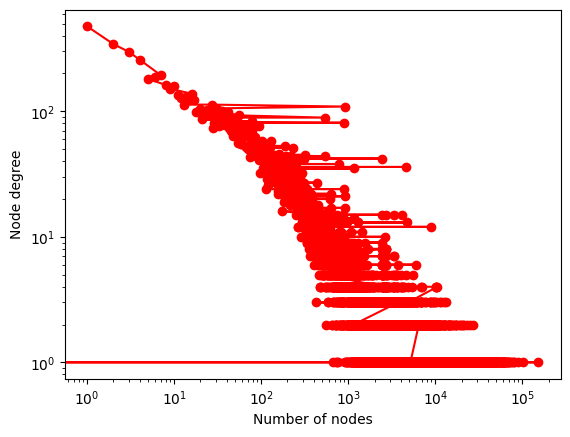
\includegraphics[width=\linewidth]{images/out-degree-distribution-loglog.png}
    \caption{Log-log scale degree distribution for game-game network.}
    \label{fig:figure1}
  \end{subfigure}
  \hspace{0.05\linewidth}
  \begin{subfigure}{0.45\linewidth}
    \centering
    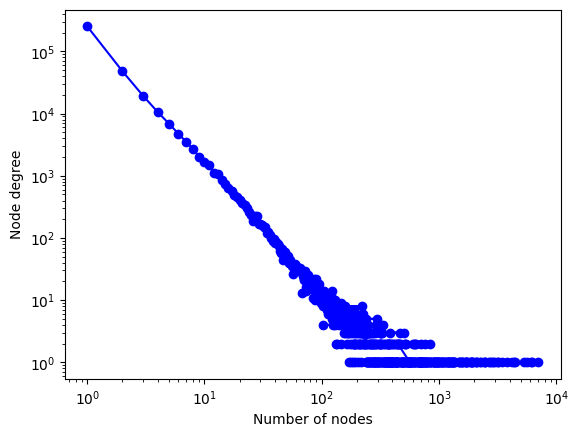
\includegraphics[width=\linewidth]{images/user-game-degree-distribution-loglog.png}
    \caption{Log-log scale degree distribution for user-game network.}
    \label{fig:figure2}
  \end{subfigure}
  \caption{Node degree distribution for the game-game and user-game networks.}
  \label{fig:figures}
\end{figure}

Four different variations of centrality were measured for the game-game network: degree, PageRank, hubs and authorities (HITS), and betweenness. Analysing the degree centrality of each of the nodes reveals Seterra is the most popular game using both in-degree and out-degree. This is followed by Celeste, Super Mario 64, Minecraft (Classic), Super Mario Bros., Mario Kart 8 Deluxe, Bee Movie Game (DS), New Super Mario Bros., Super Mario World, and Pac-Man. The game with the highest betweenness centrality is Celeste. The developer with the highest average betweenness centrality is Matt Makes Games Inc., whom are famous for developing Celeste. Furthermore the developers for Seterra, Outlast, Super Smash Bros. Ultimate, and Pringles have the highest average betweenness centrality. Other types of centrality produce similar results to the degree centrality. 


The user-game graph provides a secondary view on the games and users of speedrun.com. A directed bipartite graph was created with games and users as nodes, and edges determined by if a user has played a given game. This network has a total of 366,747 nodes and 668,788 edges. This bipartite graph has a density of $9.94 \times 10^{-6}$ and an average clustering coefficient of 0.496. There is a similar high degree distribution to the game-game network, but the user-game network has a straighter line in the log-log graph.

\subsection{Community Detection and Evaluation}

\renewcommand{\arraystretch}{1.2}
\begin{table}[h]
    \centering
    \begin{tabular}{|*{5}{C|}}
        \hline
        \textbf{Network Name} & \textbf{Algorithm Name} & \textbf{Modularity} & \textbf{Performance} & \textbf{Coverage} \\ \hline
        \multirow{3}{*}{Game-Game}  & Louvain & 0.400 & 0.697 & 0.470\\ \cline{2-5}
                                    & Infomap & 0.312 & 0.947 & 0.703 \\ \cline{2-5}
                                    & CNM & 0.275 & 0.360 & \cellcolor{CellHighlight}0.845 \\ \hline
        \multirow{3}{*}{User-Game}  & Louvain & \cellcolor{CellHighlight}0.716 & \cellcolor{CellHighlight}0.965 & 0.772 \\ \cline{2-5}
                                    & Infomap & 0.682 & 0.868 & 0.812 \\ \cline{2-5}
                                    & CNM & 0.682 & 0.911 & 0.827\\ \hline
    \end{tabular}
    \caption{Comparison of modularity, performance, and coverage on Game-Game and User-Game networks.}
    \label{tab:networks}
\end{table}

\vspace{-20pt}
\begin{figure}[h]
    \centering
    \begin{subfigure}{0.3\linewidth}
        \centering
        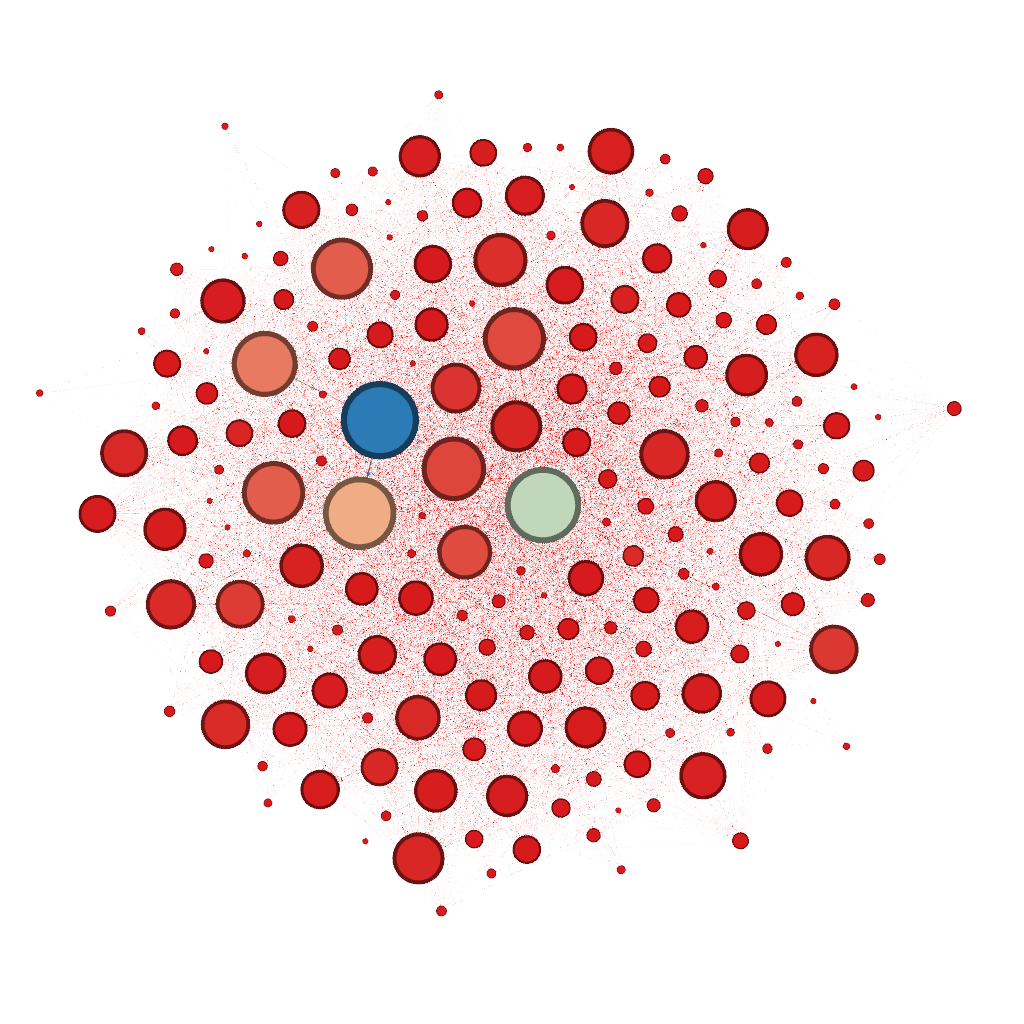
\includegraphics[width=\linewidth]{images/sub_bipartite_communities_num_games.png}
        \caption{Louvain algorithm}
        \label{fig:figure1}
    \end{subfigure}
    \hspace{0.02\linewidth}
    \begin{subfigure}{0.3\linewidth}
        \centering
        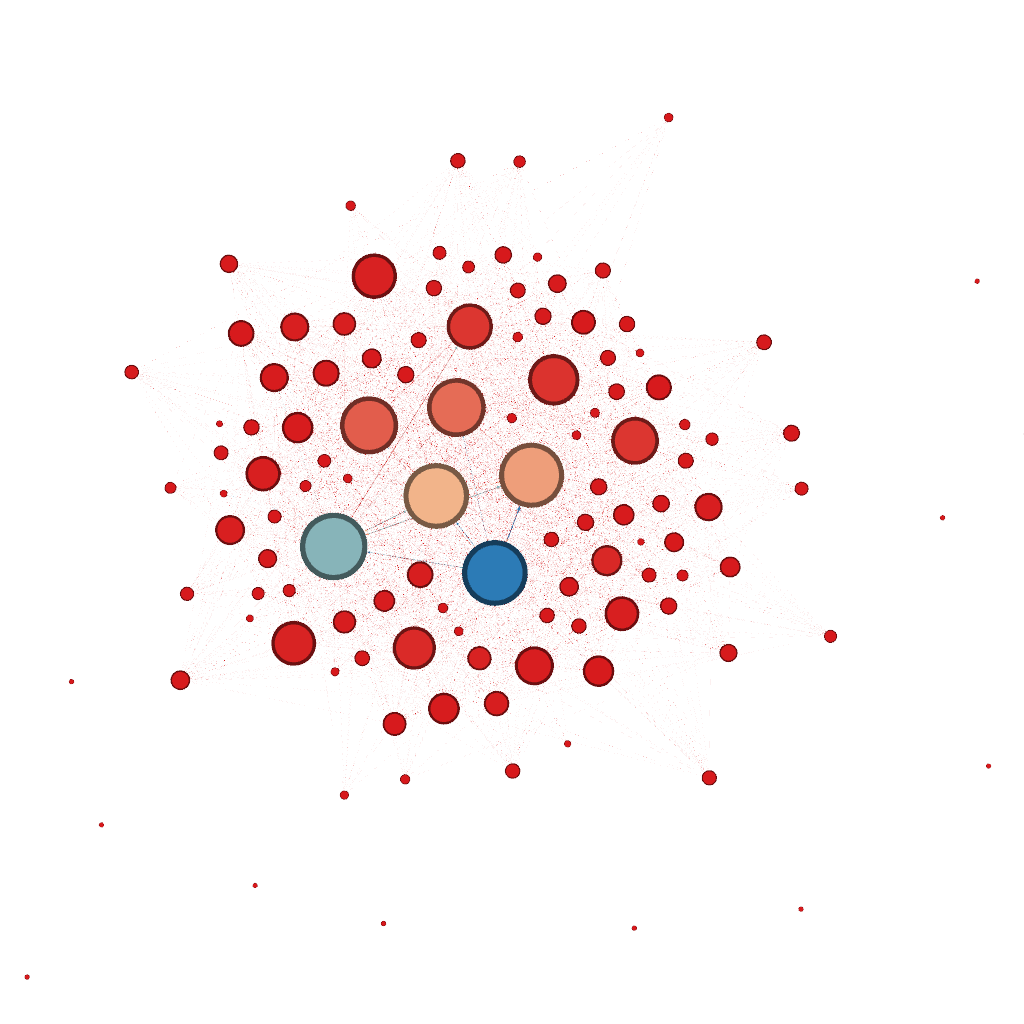
\includegraphics[width=\linewidth]{images/infomap_communities_num_games.png}
        \caption{Infomap algorithm}
        \label{fig:figure2}
    \end{subfigure}
    \hspace{0.04\linewidth}
    \begin{subfigure}{0.3\linewidth}
        \centering
        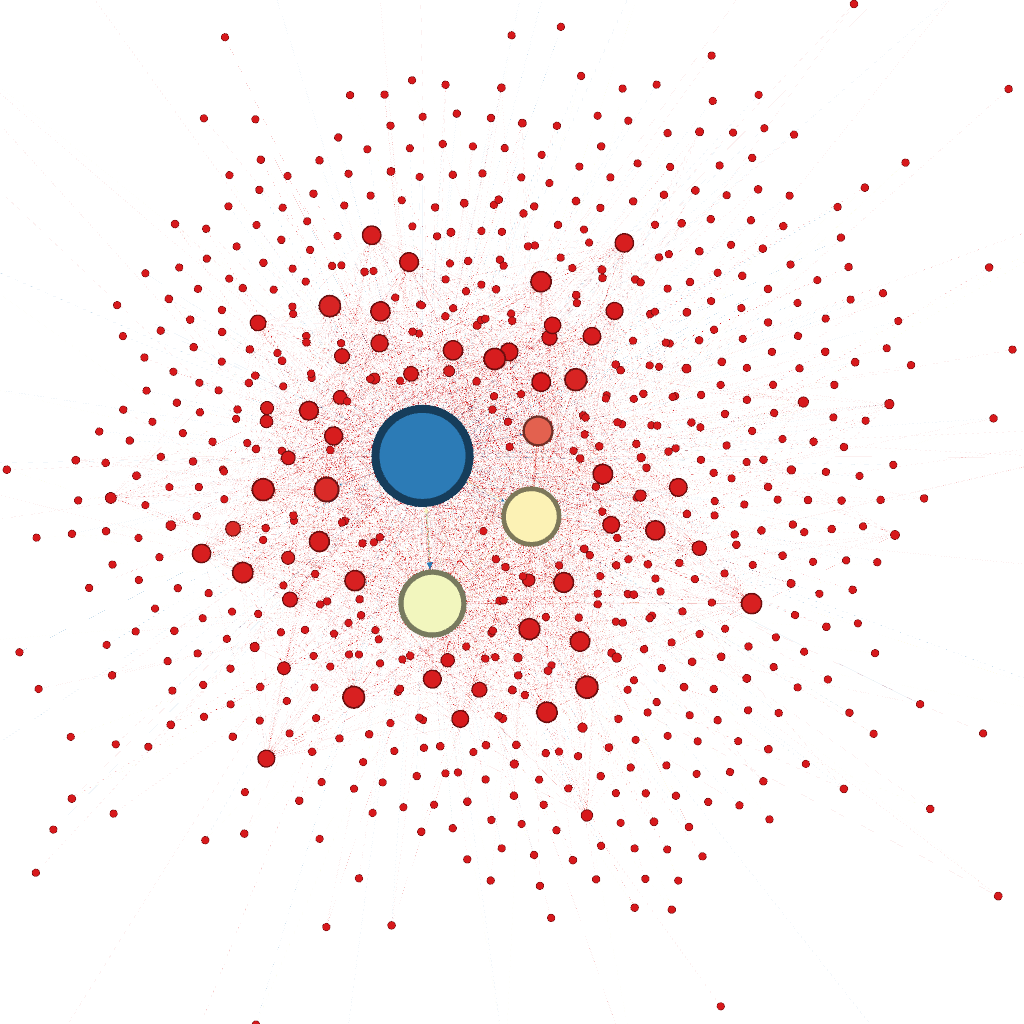
\includegraphics[width=\linewidth]{images/cnm_communities_num_games.png}
        \caption{CNM algorithm}
        \label{fig:figure2}
    \end{subfigure}
    \caption{Meta-networks of the Louvain, Infomap, and CNM algorithms on the user-game network.}
    \label{fig:figures}
\end{figure}

The Louvain, Clauset Newman Moore (CNM), and Infomap community detection algorithms provided mixed results on the game-game network. With an average modularity of 0.329. Louvain produces the highest modularity score of 0.4, whereas Clauset-Newman-Moore and Infomap algorithms produce a modularity score of 0.275 and 0.312 respectively. The Clauset-Newman-Moore algorithm produced the highest coverage of 0.845 and the lowest performance of 0.360. Infomap produces by far the best performance of 0.947 and an intermediate value of coverage and modularity when compared to the other algorithms.


Investigating the communities produced by the Louvain algorithms shows that the contents are somewhat dissimilar. Community number 23 has a number of games z-score of 16.5 with the next largest community having a z-score of 1.84. Community 23 contains over half of all games on speedrun.com. The games within this community are not very similar, ranging over many game series, platforms, decades, and genres. Community 8 of the game-game network could be categorised as video games that are available on web/mobile platforms. However, this not consistent upon including less popular games. This is a trend for most of the communities, especially for those with games that are massively popular. Some communities differ from the majority, containing a focused set of games. For example, community 27 contains 168 games with most related to the LEGO franchise or science fiction franchises such as Spider-Man, Batman, The Matrix, or Ben-10. Overall most communities in the game-game network found via the Louvain algorithm contain weakly linked video games. 


Community detection algorithms on the bipartite user-game network produced significantly better performance in all metrics. The Louvain algorithm produced 1,234 communities with a modularity of 0.716. The number of communities was reduced by removing all but the largest connected component. The largest connected component contained 364,123 out of 367,747 nodes, or 99\% of the total. Other connected components did not contain many users, with an average 2.53 nodes per connected component. By removing 2,624 nodes from the user-game network, the number of communities reduced from 1,234 to 198, while the modularity score remained at 0.716. Communities in the user-game network have on average 1,685 users and 153 games. The largest community (number zero) has 30,327 users and 2,362 games. Similarly, community 2 contains the highest number of games with 7,388 games and 20,530 users. Although the majority of communities have a consistent ratio of users to games, some communities have a low ratio considering the number of users within that community. 


The largest community in the user-game network (community one) appears to be organised around games that were originally released on platforms like the Nintendo Wii, Nintendo Switch, and Nintendo 64. Community zero follows this trend as most games were released for the Nintendo Entertainment System and Super Nintendo Entertainment System. Community two is another example of games categorised by their platform, with most video games exclusively available on the web or mobile. Several communities appear to be each related to a single entity or game franchise. For example, community four almost entirely contains games from the ROBLOX franchise, and communities six, eight, and ten containing games related to Minecraft. Some communities appear to be characterised by the mechanics of the games therein, for example community seven containing games like Portal, Refunct, Mirror's Edge, and Half-Life. Open-world video games such as Grand Theft Auto V, Need for Speed: Carbon, and Just Cause 3 are categorised together. Similarly, horror games like Five Nights at Freddy's, Hello Neighbour, and Poppy Playtime are grouped together in community 13. Some communities have a small number of games with a single incredibly popular game. Community 26 contains only 17 games and 3,495 users with the most popular game being Pou with 2,384 players compared to 889 players for Temple Run 2. The games with the highest betweenness centrality of a community are usually the most popular games in that community.


Most communities have similar demographics to the larger network. There are only 29 communities where the top demographic is not the United States or No Country Specified. All of these communities have a negative z-score of number of users. In most communities the demographic that has the largest difference between their representation in the overall game-user network and their representation in a community is usually the most popular demographic. 

\subsection{Game Recommendation System}

The content filtering recommendation method produced results with a maximum F1-score of 0.557 at 20 recommendations. Recall increases linearly with the number of recommendations, and the best combination of precision and recall occurs at 5 recommendations. Requesting game recommendations using a game in a well-known game series returns other entries of the original game series. The recommended games also usually contains games with similar game mechanics and genres. For example, requesting recommendations for Call of Duty: Black Ops III Zombies produces recommendations for games within the Call of Duty franchise (Call of Duty: Black Ops II Zombies), games within the genre of Zombies (Resident Evil 2, Outlast), and overall popular games (Grand Theft Auto V). 


The collaborative filtering method returns similar recommendations to the content filtering method. There is empirically higher diversity in the recommendations from the collaborative method compared to the content filtering method. For example, for a user that has played The Legend of Zelda: A Link to the Past, the collaborative filtering method recommends Nintendo games from most decades (such as Super Mario 64 for the N64, Mario Kart 8 Deluxe for the Nintendo Switch), and popular games (like Celeste). When inputting the same game to the content filtering method, the recommendations are focused on Nintendo games from the same era (such as Super Mario Bros. and The Legend of Zelda.